\documentclass[sn-basic]{sn-jnl}% Default

% \documentclass[default,lineno,sn-basic]{sn-jnl}% Default
% \documentclass[default,iicol]{sn-jnl}% Default with double column layout

\usepackage{graphicx}%
\usepackage{multirow}%
\usepackage{amsmath,amssymb,amsfonts}%
\usepackage{amsthm}%
\usepackage{mathrsfs}%
\usepackage[title]{appendix}%
\usepackage{xcolor}%
\usepackage{textcomp}%
\usepackage{manyfoot}%
\usepackage{booktabs}%
\usepackage{algorithm}%
\usepackage{algorithmicx}%
\usepackage{algpseudocode}%
\usepackage{listings}%


%% as per the requirement new theorem styles can be included as shown below

\newtheorem{theorem}{Theorem}%  meant for continuous numbers
%%\newtheorem{theorem}{Theorem}[section]% meant for sectionwise numbers
%% optional argument [theorem] produces theorem numbering sequence instead of independent numbers for Proposition
\newtheorem{proposition}[theorem]{Proposition}% 
%%\newtheorem{proposition}{Proposition}% to get separate numbers for theorem and proposition etc.

\newtheorem{example}{Example}%
\newtheorem{remark}{Remark}%

\newtheorem{definition}{Definition}%

\raggedbottom
%%\unnumbered% uncomment this for unnumbered level heads

\begin{document}

\title[Article Title]{Area-Throughput Efficient Implementations of CRAFT Cipher For Internet of Vehicles - v1.6.0}

\author[1,2]{\fnm{Jiahao} \sur{Xiang}}\email{simple.xjh@qq.com}
\author*[1,2]{\fnm{Lang} \sur{Li}}\email{lilang911@126.com}

\affil*[1]{\orgdiv{College of Computer Science and Technology}, \orgname{Hengyang Normal University}, \orgaddress{\city{Hengyang}, \postcode{421002},  \country{China}}}

\affil[2]{\orgdiv{Hunan Provincial Key Laboratory of Intelligent Information Processing and Application}, \orgname{Hengyang Normal University}, \orgaddress{ \city{Hengyang}, \postcode{421002}, \country{China}}}

\abstract{
    \textbf{Purpose:} With extraordinary growth in the Internet of Vehicles (IoV), the amount of data exchanged between IoV devices is growing at an unprecedented scale. Most of the IoV devices need instant response and real-time security to ensure the safety of users. The CRAFT cipher that is a lightweight block cipher for low-area can be used in IoV devices. In order to better adapt to these environment, the objective of this paper is to explore opportunities to optimize area and throughput for CRAFT cipher targeted for low-resource IoV devices.
    \textbf{Methods:} A novel compact CRAFT implementation is proposed in serialized fashion to achieve a small hardware footprint. We propose novel unrolled structure of CRAFT cipher for the high throughput feature.
    \textbf{Results:}The results on Artix-7 show that ...
    \textbf{Conclusion:} Hence, our works let CRAFT cipher more suitable for IoV devices.
}

\keywords{Lightweight block cipher, Internet of Vehicles, Field-programmable gate array(FPGA), Low-area, High-throughput}


\maketitle

\section{Introduction}\label{sec1}

Internet of Vehicles (IoV) is an emerging concept in intelligent transportation systems (ITS) to enhance the existing capabilities of VANETs by integrating with the Internet of Things (IoT) \cite{bib13}. As IoT technology continues to advance, IoV technology is also making great progress. But the same security issues that exist in IoT are also were introduced into IoV. At the some time, IoV involves a huge amount of dynamic real-time critical data so its security is a major concern.

Lightweight cryptography is a subfield of cryptography that aims to provide solutions tailored for resource-constrained devices \cite{bib12}. It can provides security with low resource consumption and low delay in IoV environment.

In this work, we propose the three architectures of FPGA implementations for the CRAFT \cite{bib5},  respectively Round based, Serial, and Loop unrolled. This allows IoV practitioners to select the architectures that best suit their needs. The contributions of this article can be summarized as follows.

The rest of this article is organized as follows. Section~\ref{sec2} presents specification of CRAFT; the proposed the three architectures of FPGA implementations for the CRAFT are present in Section 3; Section 4 presents the implementation results, analysis, and comparison with other similar works; finally, the work is concluded in Section 5.


\section{Specification of CRAFT}\label{sec2}

All notations used in this paper are shown in Table~\ref{tab1}. CRAFT is a lightweight tweakable block cipher made out of involutory building blocks. It consists of a 64-bit block, a 128-bit key, and a 64-bit tweak. In this cipher, a 64-bit input plaintext P is transformed into a 64-bit output ciphertext C using a 128-bit key K and a 64-bit tweak T. Figure~\ref{fig1} shows the structure of CRAFT.

\begin{table}[h]
    \caption{Notations used in this paper}\label{tab1}%
    \begin{tabular*}{\textwidth}{@{\extracolsep\fill}lcccccc}
        \toprule
        Notation   & Description                                 \\
        \midrule
        $TK$       & 64-bit tweakeys                             \\
        $RC_i$     & 64-bit round constant in the $i^{th}$ round \\
        $R_i,R'_i$ & Round function                              \\
        $\oplus$   & Bit-wise sum (XOR)                          \\
        \botrule
    \end{tabular*}
\end{table}

\begin{figure}[h]%   
    \caption{Structure of CRAFT}\label{fig1}
    \centering
    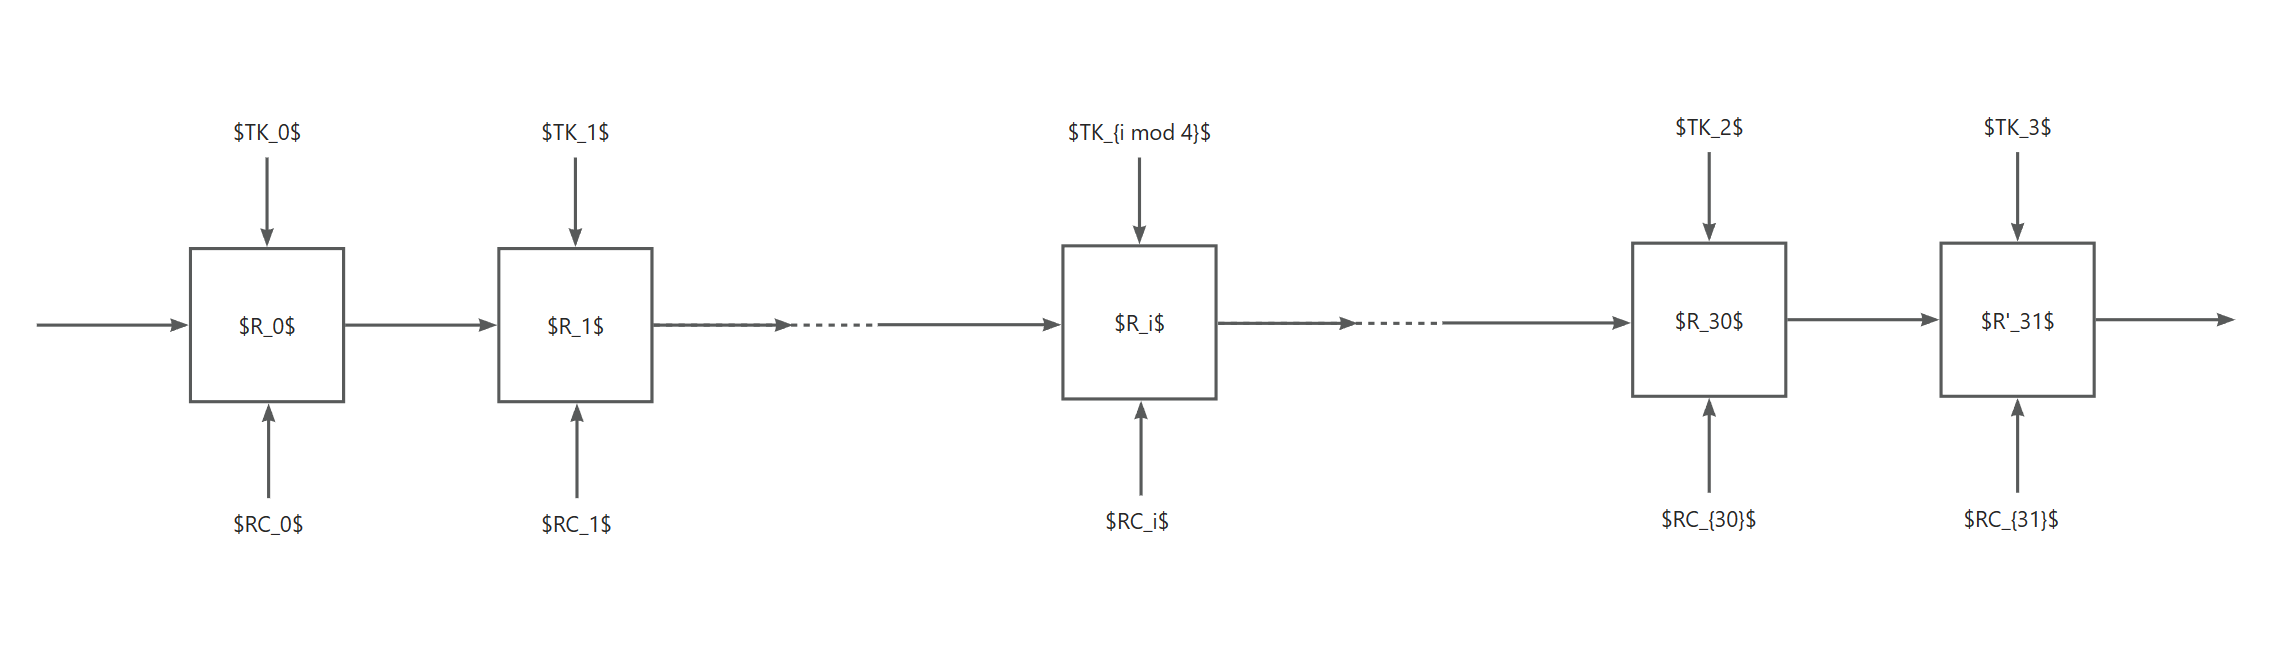
\includegraphics[width=\textwidth]{struct_of_craft.png}
\end{figure}


\section{CRAFT Implementation}\label{sec3}

In order to achieve efficient area and throughput, we optimize the components of craft for the first time and propose three implementation architectures, respectively Round based, Serial, and Loop unrolled. Proposed architectures are implemented on the Xilinx FPGA board using the Vivado v2023.1. FPGA platforms - Artix-7 (xc7a100tcsg324-1) are used to get a clear idea about implementation and performance of the proposed designs.

\subsection{Round Based Architecture}\label{subsec1}
As no FPGA implementation of the round based architecture is given in \cite{bib5}, we implement the architecture presented in \cite{bib5} for the first time. Figure~\ref{fig2} is Round-based design architecture of CRAFT. In terms of area, the consumption of each component of the algorithm is shown in Table~\ref{tab2}. The larger part of the footprint is the intermediate register state and the non-linear component sbox. In terms of throughput, The critical path is from the control register to the intermediate value register state, which has a delay of 5.2ns. the calculated maximum throughput rate is 382Mbit/s.


\begin{figure}[h]%   
    \caption{Structure of CRAFT}\label{fig2}
    \centering
    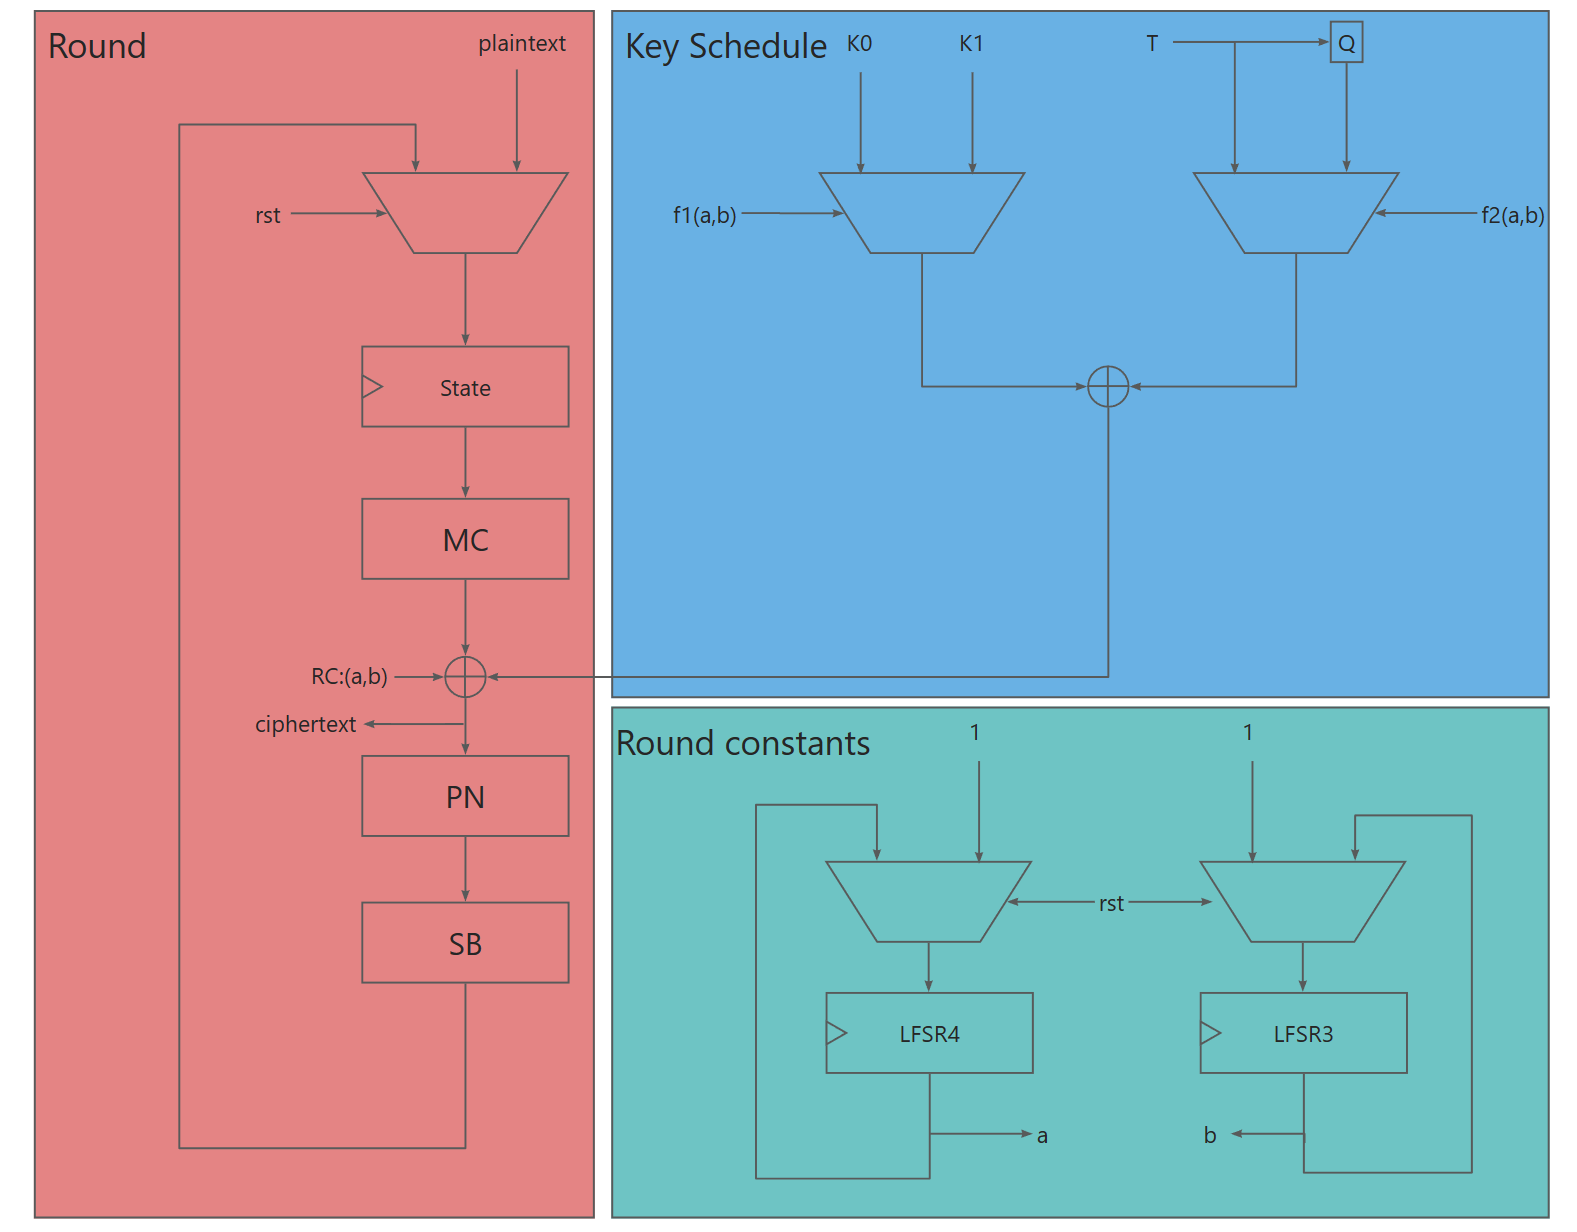
\includegraphics[width=\textwidth]{round_based_design.png}
\end{figure}

\begin{table}[h]
    \caption{Area consumption of Round based design}\label{tab2}%
    \begin{tabular*}{\textwidth}{@{\extracolsep\fill}lcccccc}
        \toprule
        &LUT&	FF&	Slice                                \\
        \midrule
        Key Schedule &	64&	0&	22                           \\
        Round Constant&	2&	7&	2 \\
        Sbox * 4&	8&	0&	4                             \\
        Round (include  Sbox * 16)&	84&	0&	28                        \\
        All (include control)&	182&	144&	56                     \\
        \botrule
    \end{tabular*}
\end{table}

\subsection{Serial Architecture}\label{subsec2}
Compared to round-based architecture, serial architecture are able to reuse components and significantly reduce area usage, e.g., the number of sboxes is reduced from 16 to 1. The clock gating technique is also used to enable each component and reduce the energy consumption of encryption. Our proposed architecture is presented in Figure~\ref{fig3}. The design includes one Sub-Box, one 4-bit Mix-columns, two register banks for storing keys (called Key-Register) and plaintext (called State-Register), which also act as temporary registers for storing the intermediate results. In order to store intermediate results into State-Register bank, the design has one feedback paths. PermuteNibbles is included in State-Register bank. It is noticeable that since the execution of permute requires 64-bit, in order to reuse the State-Register block, we change the order of execution of Sub-Box and Permute. And the first round of encryption process through the control signal to avoid Permute operation, to ensure the correctness of the encryption algorithm.

\begin{figure}[h]%   
    \caption{Serial architecture of CRAFT}\label{fig3}
    \centering
    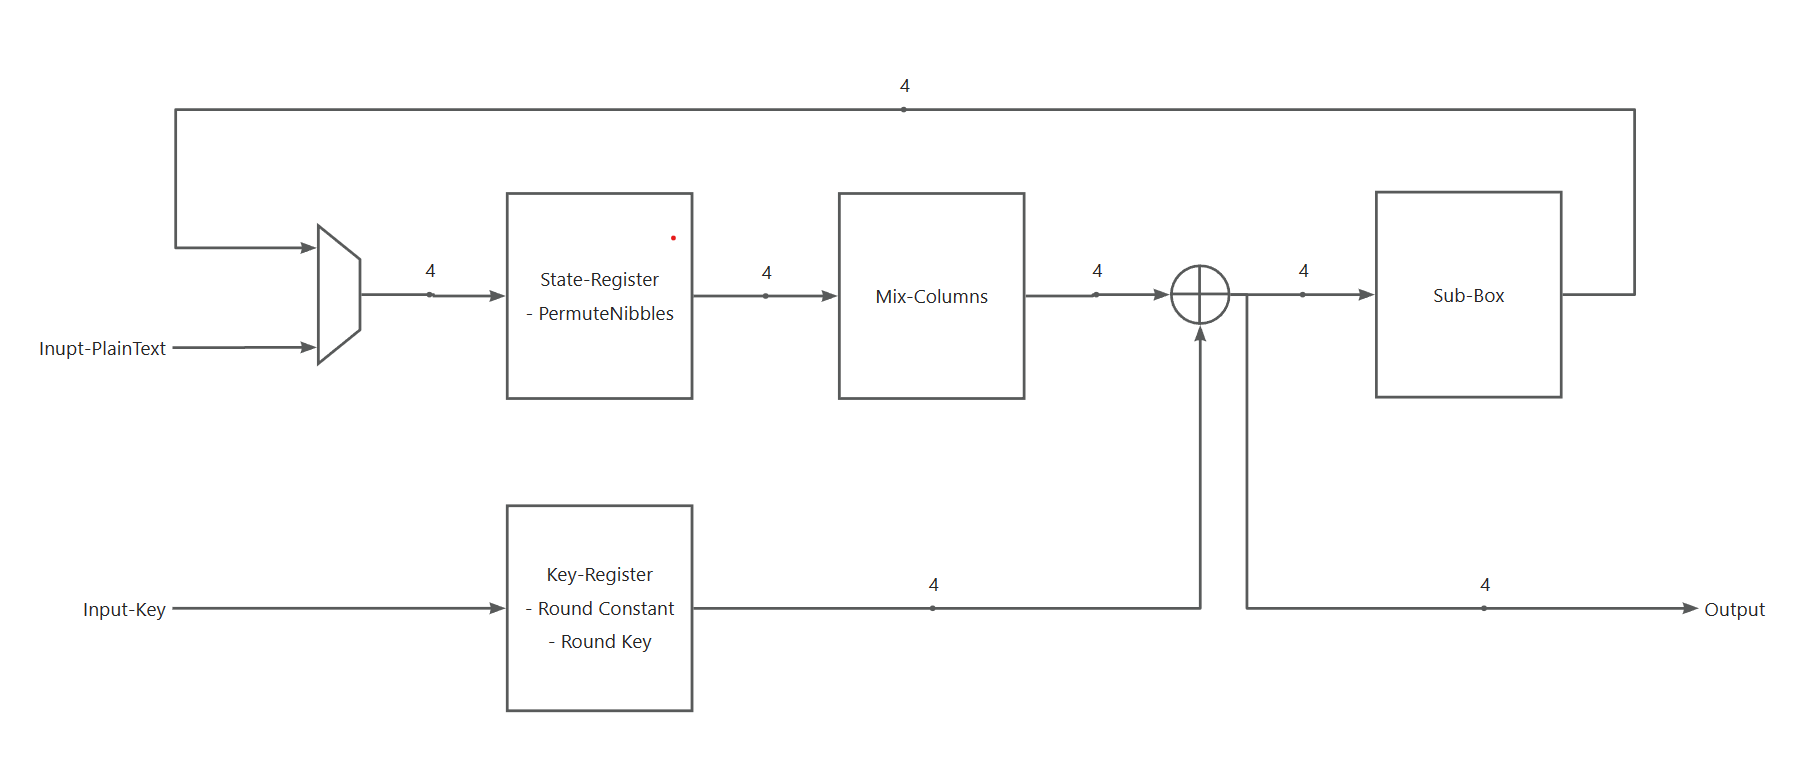
\includegraphics[width=\textwidth]{serial_design.png}
\end{figure}

The finite-state machine (FSM) of serial architecture is shown in Figure~\ref{fig4}. The initial key and plaintext are stored in Key-Register and State-Register at the same time. After the Store, the key is expanded in Key Schedule. In Mix Columns, one column of State-Register stores in the Mix Columns registers that take four clock cycles for execution Mix-Columns over one column. In Add Key, the stored data in Mix Columns's registers are sent back to State-Register followed by XORing with keys and Throughing the sbox component in another four clock cycles. Permute executes in one clock cycle inside the State-Register.

\begin{figure}[h]%   
    \caption{Finite-state machine for serial architecture}\label{fig4}
    \centering
    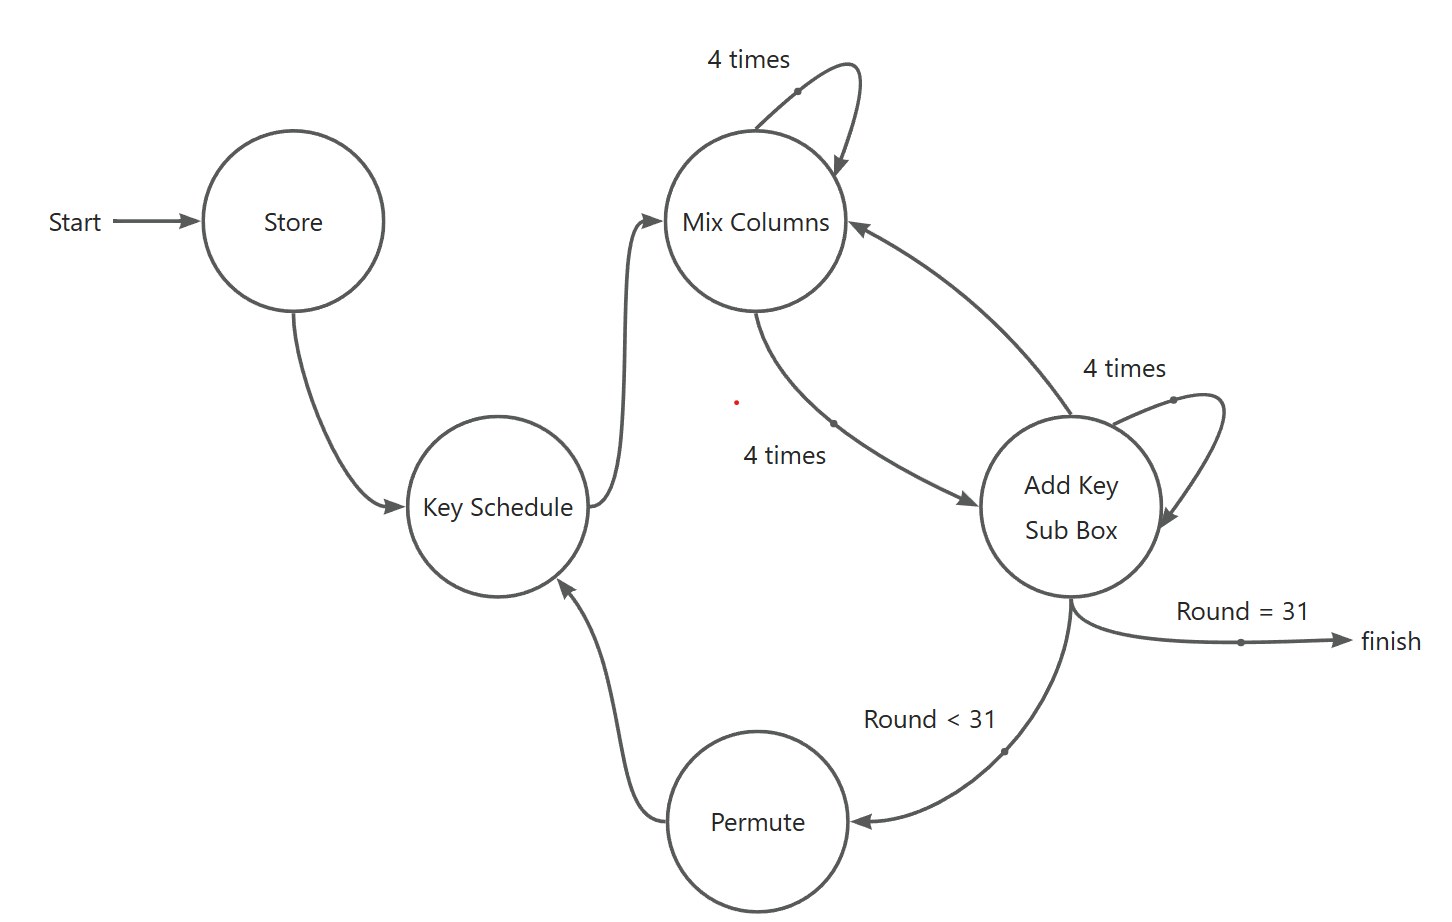
\includegraphics[width=\textwidth]{serial_fsm.png}
\end{figure}

Additionally, the dynamic power consumption of the encryption is reduced by using clock gating.The clock gating is separately applied on State Register, Key Register and Mix Columns. For instance, the most power consumption is saved during the Key Schedule phase; the clock of State Register and Mix Columns is disabled to save power because these two blocks are not used in the Key Schedule phase. The timing diagram of the proposed design with the clock gating technique is shown in Figure~\ref{fig5}.

\begin{figure}[h]%   
    \caption{Timing diagram for serial architecture}\label{fig5}
    \centering
    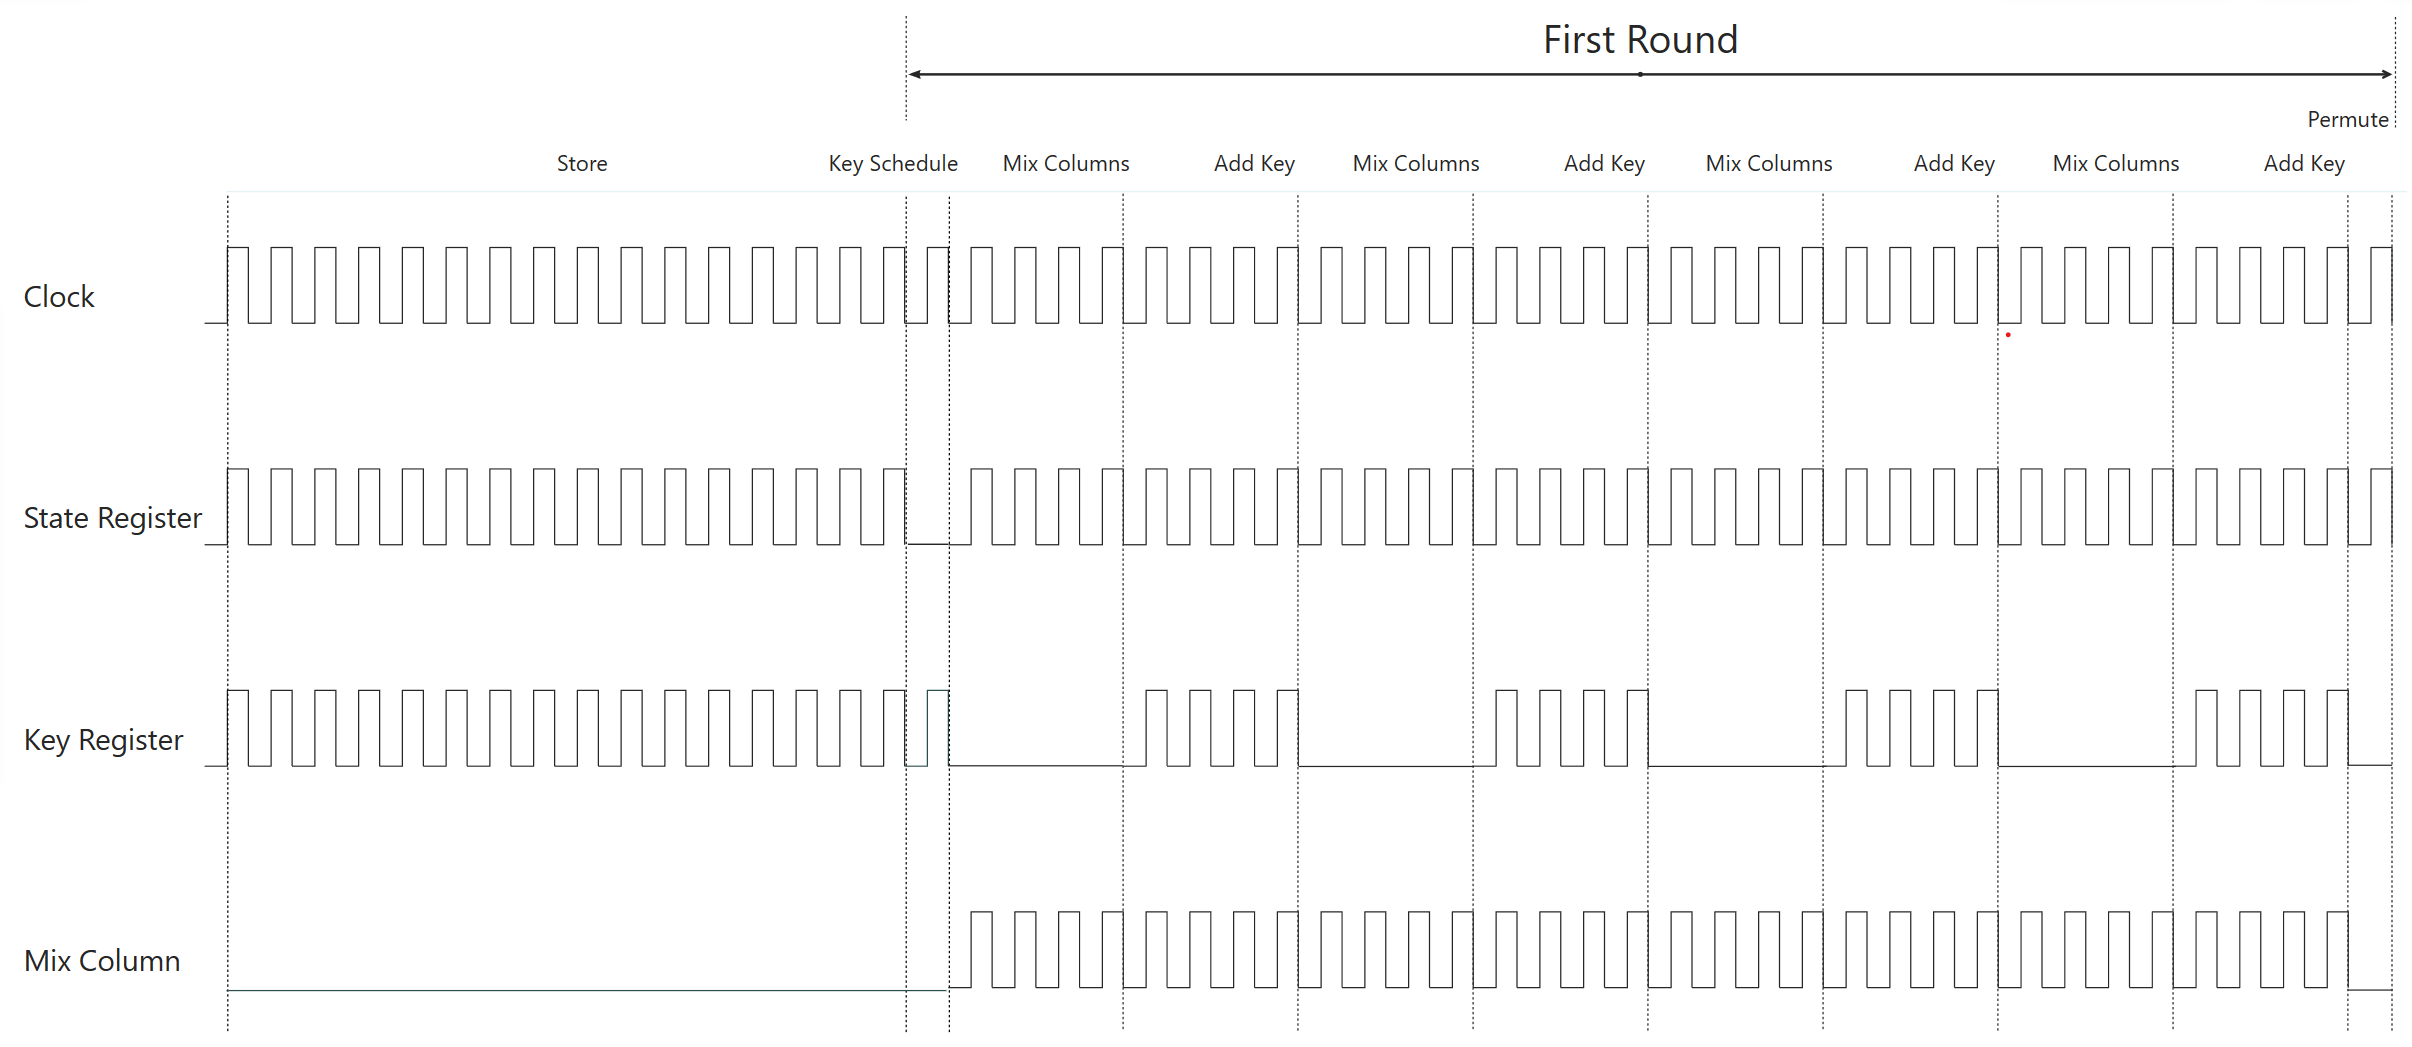
\includegraphics[width=\textwidth]{serial_time.png}
\end{figure}

\subsubsection{Sub Box Optimization }\label{subsubsec1}
Sub Box provides a confusing characteristic for the entire encryption algorithm, however it requires a large amount of area. There are different methods of implementation of Sub Box. The most popular implementation is using a lookup table (LUT), such as \cite{bib17}. However it uses a lot of flip-flop, which will bring a lot of area consumption. Using S-Box's equivalent logical expression for this will reduce area consumption, such as \cite{bib15}, \cite{bib16}.

SAT solvers can be used to find S-Box that satisfy certain implement, such as being resistant to software or hardware implement.
In more detail, the S-Box implement can be encoded as Boolean constraints by representing the S-Box as a truth table and then using Boolean variables to represent the input and output bits of the S-Box.
The constraints can then be formulated based on the desired implement of the S-Box.
Once the S-Box implement are encoded as Boolean constraints, a SAT solver can be used to find a satisfying assignment to these constraints, which corresponds to an S-Box that satisfies the desired implement.

The gate equivalent complexity(GEC) of a SAT instance is the number of logical gates required to implement the Boolean formula that represents the instance.
GEC can be calculated by converting the Boolean formula into a circuit of logical gates, such as AND, OR, and NOT gates.
The number of gates in the circuit corresponds to the GEC of the instance.

In our design, we optimize and use GEC encoding scheme of \cite{bib16} to implement the S-Box.
Our encoding scheme as follows in Equation~\ref{eq1}:

\begin{align}
    \forall i \in \{0,1,\ldots ,K-1\}: \nonumber                                                                  \\
    T_i & = F_{if} (BB_i[0], \thicksim (Q_{4i} \cdot Q_{4i+1}) \cdot \thicksim Q_{4i+2} \cdot Q_{4i+3}) \nonumber \\
        & \quad + F_{if} (BB_i[1], Q_{4i+2} \cdot (Q_{4i} + Q_{4i+1})) \nonumber                                  \\
        & \quad + F_{if} (BB_i[2], Q_{4i} \cdot Q_{4i+1} \cdot Q_{4i+2}) \nonumber                                \\
        & \quad + F_{if} (BB_i[3], Q_{4i+2}) + F_{if} (BB_i[4], Q_{4i}) \nonumber                                 \\
        & \quad + F_{if} (BB_i[5], Q_{4i} \cdot Q_{4i+1}) \nonumber                                               \\
        & \quad + F_{if} (BB_i[6], Q_{4i} + Q_{4i+1}) + F_{if} (BB_i[7], \max). \label{eq1}
\end{align}

where $K$ is numbers of the logical gates, $Q_{4i}-Q_{4i+3}$ is the input of the $i^{th}$ logical gate, $T_i$ is the output of the $i^{th}$ logical gate, and $F_{if}$ is a function that returns the value of the second argument if the first argument is true and returns the value of zero otherwise.
The value of $max$ is all one's in the binary expression, which is represented logically as an inverse.
$BB_i$ represents the type of the $i^{th}$ logical gate, which is a 8-bit binary number. The different types of logical gate used in this encoding scheme are listed in Table~\ref{tab3}.


\begin{table}[h]
    \caption{Encoding of different types of logical gate}\label{tab3}%
    \begin{tabular*}{\textwidth}{@{\extracolsep\fill}lcccccc}
        \toprule
        logical expression & $BB_i$[0:7] & gate type \\
        \midrule
        $Q_0 \oplus Q_1$ & 0 0 0 0 0 0 1 0 & XOR \\
        $\sim (Q_0 \oplus Q_1)$ & 0 0 0 0 0 0 1 1 & XNOR \\
        $Q_0 \land Q_1$ & 0 0 0 0 0 1 0 0 & AND \\
        $\sim (Q_0 \land Q_1)$ & 0 0 0 0 0 1 0 1 & NAND \\
        $Q_0 \lor Q_1$ & 0 0 0 0 0 1 1 0 & OR \\
        $\sim (Q_0 \lor Q_1)$ & 0 0 0 0 0 1 1 1 & NOR \\
        $\sim Q_0$ & 0 0 0 0 1 0 0 1 & NOT \\
        $\sim Q_1$ & 0 0 0 0 1 0 1 1 & NOT \\
        $\sim Q_2$ & 0 0 0 1 0 0 0 1 & NOT \\
        $Q_0 \oplus Q_1 \oplus Q_2$ & 0 0 0 1 0 0 1 0 & XOR3 \\
        $\sim (Q_0 \oplus Q_1 \oplus Q_2)$ & 0 0 0 1 0 0 1 1 & XNOR3 \\
        $Q_0 \land Q_1 \land Q_2$ & 0 0 1 0 0 0 0 0 & AND3 \\
        $\sim (Q_0 \land Q_1 \land Q_2)$ & 0 0 1 0 0 0 0 1 & NAND3 \\
        $Q_0 \lor Q_1 \lor Q_2$ & 0 1 1 1 0 1 1 0 & OR3 \\
        $\sim (Q_0 \lor Q_1 \lor Q_2)$ & 0 1 1 1 0 1 1 1 & NOR3 \\
        $\sim ((Q_0 \land Q_1) \lor (\sim (Q_2 \lor Q_3)))$ & 1 0 1 1 0 0 0 0 & MAOI1 \\
        $\sim (\sim (Q_0 \land Q_1) \land ((Q_2 \lor Q_3)))$ & 1 0 1 1 0 0 0 1 & MOAI1 \\
        \bottomrule
    \end{tabular*}
\end{table}

The optimized architecture of S-Box is shown in Equation~\ref{eq2}, where $X_0-X_3$ is the input of the S-Box and $Y_0-Y_3$ is the output of the S-Box. The proposed architecture of S-Box is implemented by four MOAI1 gates, three MAOI1 gates, and one AND3 gate. This module of the proposed S-Box reduced the area by 28.9\% with \cite{bib15} (based on gate equivalent estimation on UMC 180nm library).

\begin{align}
    T_0 &= \text{MAOI1}(X_0, X_1, X_0, X_1) \nonumber \\
    T_1 &= \text{AND3}(X_3, X_2, X_3) \nonumber \\
    T_2 &= \text{MAOI1}(X_1, X_2, X_0, X_3) \nonumber \\
    T_3 &= \text{MOAI1}(X_1, X_0, X_2, X_2) \nonumber \\
    T_4 &= \text{MOAI1}(X_3, T_0, T_3, T_3) \nonumber \\
    T_5 &= \text{MOAI1}(T_3, T_0, X_0, T_1) \nonumber \\
    T_6 &= \text{MAOI1}(X_0, T_0, X_3, T_0) \nonumber \\
    T_7 &= \text{MOAI1}(X_0, T_1, T_2, T_2) \nonumber \\
    Y_0 &= T_5 \nonumber \\
    Y_1 &= T_7 \nonumber \\
    Y_2 &= T_6 \nonumber \\
    Y_3 &= T_4 \label{eq2}
\end{align}

\subsection{Loop Unrolled Architecture}\label{subsec3}

\section{Implementation Results And Analysis}\label{sec4}

\section{Conclusion}\label{sec5}

\bibliography{sn-bibliography}% common bib file
%% if required, the content of .bbl file can be included here once bbl is generated
%%\input sn-article.bbl

\end{document}
